% ucpqc -- technical report
% Compile: latexmk -pdf ucpqc_report.tex   (or: pdflatex twice)
% Replace \author{} below with your name.
\documentclass[11pt]{article}

\usepackage[utf8]{inputenc}
\usepackage[T1]{fontenc}
\usepackage{lmodern}
\usepackage[margin=1in]{geometry}
\usepackage{amsmath,amssymb}
\usepackage{booktabs}
\usepackage{longtable}
\usepackage{array}
\usepackage{graphicx}
\usepackage{xcolor}
\usepackage{listings}
\usepackage{enumitem}
\usepackage{caption}
\usepackage{tikz}
\usetikzlibrary{positioning,arrows.meta,fit}
\usepackage[colorlinks=true,linkcolor=blue!55!black,urlcolor=blue!55!black,
            citecolor=blue!55!black]{hyperref}

\graphicspath{{../examples/plots/9/}{./}}

\definecolor{codebg}{RGB}{247,247,249}
\definecolor{kw}{RGB}{140,40,120}
\definecolor{cmt}{RGB}{90,120,90}
\definecolor{str}{RGB}{50,100,160}

\lstset{
  basicstyle=\ttfamily\footnotesize,
  backgroundcolor=\color{codebg},
  keywordstyle=\color{kw}\bfseries,
  commentstyle=\color{cmt}\itshape,
  stringstyle=\color{str},
  showstringspaces=false,
  breaklines=true,
  frame=single,
  rulecolor=\color{black!15},
  columns=fullflexible,
  keepspaces=true,
  literate={->}{{$\rightarrow$}}1 {>=}{{$\geq$}}1 {<=}{{$\leq$}}1,
}
\lstdefinestyle{py}{language=Python}
\lstdefinestyle{sh}{language=bash}
\lstdefinestyle{out}{basicstyle=\ttfamily\scriptsize,keywordstyle=\color{black}}

\newcommand{\code}[1]{\texttt{#1}}
\newcommand{\ucpqc}{\code{ucpqc}}
\newcommand{\Zq}{\ensuremath{\mathbb{Z}_q}}
\newcommand{\GF}[1]{\ensuremath{\mathrm{GF}(#1)}}

\title{\textbf{\ucpqc: An Emulation-Based Fault-Analysis Platform\\
for Post-Quantum Cryptography}\\[4pt]
\large Architecture, Detectors, Statistical Calibration, and Results}
\author{\textit{(author name)}}       % <-- replace with your name
\date{\today}

\begin{document}
\maketitle

\begin{abstract}
\noindent
\ucpqc{} is a Unicorn-based emulation platform that answers one mechanical
question at scale: \emph{if a fault is injected at this point in a post-quantum
cryptographic implementation, does the output start leaking the secret key?} It
boots real \code{pqm4}/\code{pqcrystals} Cortex-M4 firmware inside a full CPU
emulator, injects a fault at a chosen site, and runs a \emph{repertoire} of
statistical detectors on the resulting outputs to decide \textsc{leak}/ok. The
platform is deliberately scheme-agnostic: a thin \emph{profile} layer supplies
the algebra of each algorithm, while the emulator, fault injector, capture-replay
engine, detector library, and assessment engine never mention a concrete scheme.
The current build supports CRYSTALS-Dilithium (ML-DSA-44, lattice) and MAYO
(multivariate), with the KEM path (ML-KEM/Kyber) present at the scheme layer. This
report explains the whole codebase module by module, presents the recently added
\emph{statistically calibrated} verdict (per-site permutation / analytic
$p$-values combined by a sweep-wide false-discovery-rate rule, replacing hand-tuned
thresholds), and discusses the design tradeoffs and empirical results---including
the headline Dilithium mask-removal leak, the honest limits observed on MAYO, and
the emulation and parallelism cost/accuracy tradeoffs.
\end{abstract}

\tableofcontents
\bigskip

%======================================================================
\section{Introduction and Goals}
%======================================================================

Post-quantum cryptography (PQC) is being standardised (FIPS~203/204/205) and
deployed on embedded targets, where an attacker has physical access and can
inject \emph{faults}---clock glitches, voltage glitches, laser pulses---to perturb
a computation. Many PQC schemes have a structural weakness that a single
well-placed fault can expose: a masking value that must stay secret, a rejection
check that must not be bypassed, or an algebraic recombination that must not leak
an intermediate. Evaluating a protected implementation against this class of
attack by hand, one fault at a time, does not scale.

\ucpqc{} is built to make that evaluation \emph{systematic and generic}. Its
design goals, in priority order, are:

\begin{enumerate}[leftmargin=1.6em]
  \item \textbf{Solid detectors.} A \textsc{leak} verdict should be a
  \emph{calibrated} statistical decision with a false-positive guarantee, not a
  magic threshold. The platform ships a repertoire of complementary detectors
  (mean-shift, per-coordinate, subspace, algebraic-structural, distributional,
  spec-boundary) unified under one calibration mechanism.
  \item \textbf{Genericity across PQC families.} The same engine must assess
  lattice signatures, multivariate signatures, and (by construction) KEMs. Only a
  small per-scheme profile is written; everything else is shared.
  \item \textbf{Catch many fault points.} Fault sites are \emph{auto-discovered}
  by disassembly, and two fault surfaces are provided: whole-call skips and
  intra-function instruction skips.
  \item \textbf{Test protected implementations for side effects.} Because the
  emulator is deterministic and reproducible, a hardened build can be assessed the
  same way as an unprotected one.
\end{enumerate}

A deliberate scoping decision underlies the whole platform: \textbf{it decides
leak / no-leak; it does not recover keys.} This keeps the analysis cheap
(tens of traces, not millions) and the verdict interpretable, and it matches the
practical question a countermeasure designer asks: ``does this fault re-open a
key-dependent channel?''

%======================================================================
\section{Background}
%======================================================================

\subsection{The two target schemes}

\paragraph{CRYSTALS-Dilithium / ML-DSA (lattice, Fiat--Shamir with aborts).}
Signing repeatedly samples a fresh masking nonce $y$, forms the response
\[
  z \;=\; y + c\cdot s_1 \pmod{q},
\]
where $c$ is a sparse $\pm1$ challenge polynomial (expanded from the signature's
$\tilde c$ seed) and $s_1$ is part of the secret key. The nonce $y$ is a
\emph{mask}: it makes the marginal distribution of $z$ independent of the secret,
which is exactly why a plain histogram of $z$ reveals nothing. The scheme then
applies several \emph{rejection checks} ($\lVert z\rVert$, $\lVert r_0\rVert$,
$\lVert ct_0\rVert$, hint weight); if any fails, it resamples $y$ and retries. Two
fault-attack surfaces follow immediately: (i) remove the mask
($z=z+y \to z=c\cdot s_1$), and (ii) force a rejection check to accept, releasing
out-of-spec signatures. ML-DSA-44 parameters used throughout:
$q=8380417$, $n=256$ coefficients, $\ell=4$, $\tau=39$,
$\gamma_1=2^{17}$, $\gamma_2=(q-1)/88$, $\beta=78$.

\paragraph{MAYO (multivariate, Oil-and-Vinegar).}
MAYO is \emph{not} lattice-based. Its secret is a hidden ``oil'' subspace
$O\subset \GF{16}^n$. Signing fixes fresh random \emph{vinegar} variables (expanded
from a seed by SHAKE), which makes the public map linear in the oil variables, then
solves a linear system and outputs $s = v + o$ (vinegar $+$ oil). The crown-jewel
asymmetry is that \emph{if an attacker learns or fixes the vinegar}, the signing
equation becomes a solvable linear system that leaks the oil space---the key. Thus
the fault-critical operations are the vinegar seed expansion, the linear solve, and
the final recombination $s=v+o$. All arithmetic is over $\GF{16}=\GF{2^4}$.

\subsection{The fault model}
The physical faults \ucpqc{} models are \emph{instruction skip} (a fetch/execute
glitch that turns an instruction, or a whole call, into a no-op), \emph{data
corruption} (bit-flip or stuck-at on a register or memory word), and
\emph{branch inversion} (flip a condition flag). These correspond one-to-one to
the fault models in \code{faults.py} (\S\ref{sec:faults}).

%======================================================================
\section{Architecture Overview}\label{sec:arch}
%======================================================================

\ucpqc{} is layered so that scheme knowledge is confined to a single thin layer.
Figure~\ref{fig:arch} shows the stack; Table~\ref{tab:modules} lists the modules.

\begin{figure}[h]
\centering
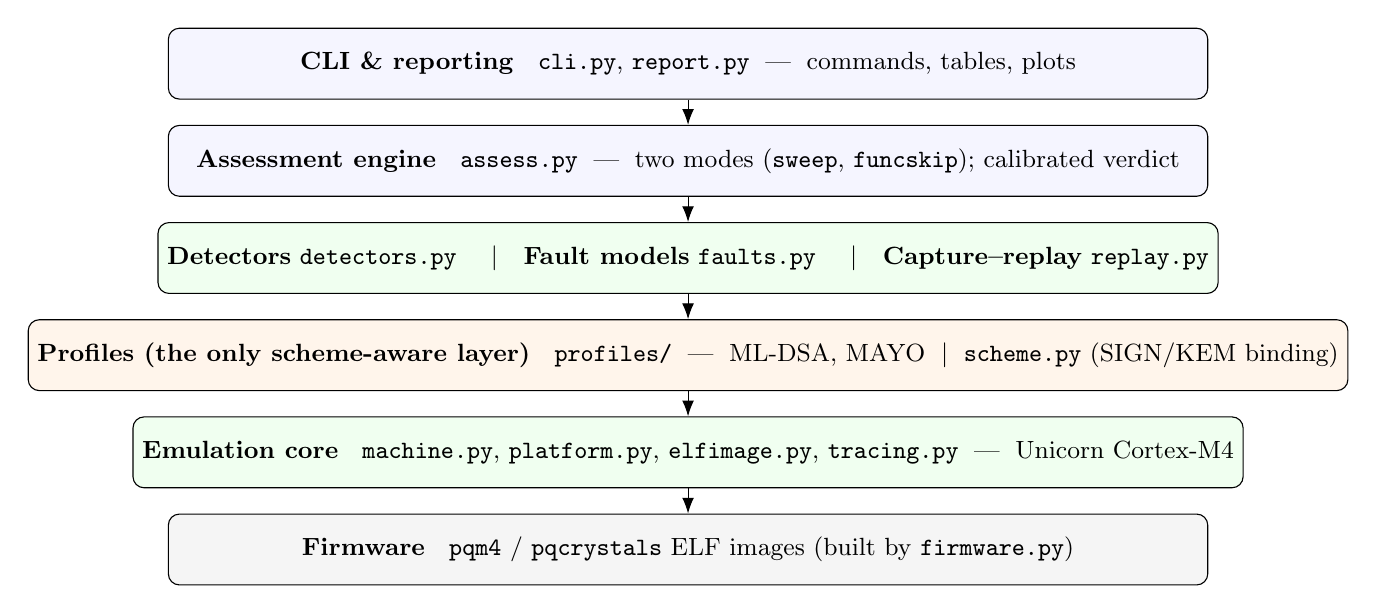
\begin{tikzpicture}[
  font=\small,
  layer/.style={draw, rounded corners, minimum width=13.2cm, minimum height=0.9cm,
                align=center, fill=blue!4},
  scheme/.style={layer, fill=orange!8},
  core/.style={layer, fill=green!6},
  node distance=3.2mm,
]
\node[layer] (cli) {\textbf{CLI \& reporting} \; \code{cli.py}, \code{report.py} \;---\; commands, tables, plots};
\node[layer, below=of cli] (assess) {\textbf{Assessment engine} \; \code{assess.py} \;---\; two modes (\code{sweep}, \code{funcskip}); calibrated verdict};
\node[core, below=of assess] (det) {\textbf{Detectors} \code{detectors.py} \quad\textbar\quad \textbf{Fault models} \code{faults.py} \quad\textbar\quad \textbf{Capture--replay} \code{replay.py}};
\node[scheme, below=of det] (prof) {\textbf{Profiles (the only scheme-aware layer)} \; \code{profiles/} \;---\; ML-DSA, MAYO \;\textbar\; \code{scheme.py} (SIGN/KEM binding)};
\node[core, below=of prof] (mach) {\textbf{Emulation core} \; \code{machine.py}, \code{platform.py}, \code{elfimage.py}, \code{tracing.py} \;---\; Unicorn Cortex-M4};
\node[layer, below=of mach, fill=black!4] (fw) {\textbf{Firmware} \; \code{pqm4} / \code{pqcrystals} ELF images (built by \code{firmware.py})};

\draw[-{Latex[length=2mm]}] (cli) -- (assess);
\draw[-{Latex[length=2mm]}] (assess) -- (det);
\draw[-{Latex[length=2mm]}] (det) -- (prof);
\draw[-{Latex[length=2mm]}] (prof) -- (mach);
\draw[-{Latex[length=2mm]}] (mach) -- (fw);
\end{tikzpicture}
\caption{Layered architecture. Scheme-specific knowledge lives only in
\code{profiles/} and \code{scheme.py}; every other layer works on instructions,
memory, and feature matrices.}
\label{fig:arch}
\end{figure}

\begin{table}[h]
\centering\small
\caption{Modules (\,$\approx$\,5{,}300 lines of Python\,).}
\label{tab:modules}
\begin{tabular}{@{}llr@{}}
\toprule
Module & Responsibility & LoC \\
\midrule
\code{machine.py}      & Cortex-M4 emulation, snapshot/restore, scratch, stub RNG, hooks & 646 \\
\code{tests/run\_tests.py} & 32-test system suite (runs on 3.12 and 3.14t)          & 523 \\
\code{cli.py}          & \code{python -m ucpqc} command front-end                    & 470 \\
\code{detectors.py}    & Feature + detector + calibration library                    & 432 \\
\code{assess.py}       & Scheme-agnostic assessment engine (two modes)               & 423 \\
\code{replay.py}       & Capture-and-replay for intra-function skips                 & 396 \\
\code{scheme.py}       & SIGN/KEM detection and API binding                          & 394 \\
\code{faults.py}       & Six fault models, injector, campaign runner                 & 357 \\
\code{tracing.py}      & Instruction/call/memory tracers, profiler, \code{Trigger}   & 341 \\
\code{firmware.py}     & \code{pqm4} build wrapper + manifest                        & 217 \\
\code{platform.py}     & MPS2-AN386 memory map + MMIO peripherals                     & 201 \\
\code{profiles/*}      & \code{AnalysisProfile} + ML-DSA + MAYO                      & 454 \\
\code{elfimage.py}     & ELF parsing / symbol lookup                                  & 163 \\
\code{report.py}       & Console table + bar-chart rendering                         & 101 \\
\bottomrule
\end{tabular}
\end{table}

%======================================================================
\section{The Emulation Core}
%======================================================================

\subsection{\code{machine.py} --- the emulated Cortex-M4}
\code{Machine} wraps a Unicorn \code{Uc} instance in Thumb/M-class mode running a
Cortex-M4 model, plus a Capstone disassembler. It provides the primitives every
higher layer relies on:

\begin{itemize}[leftmargin=1.4em]
  \item \textbf{Boot and call.} \code{boot()} runs reset $\to$ C-runtime init $\to$
  \code{main} (so \code{.bss} is zeroed and the FPU is on), then \code{call(func,
  args)} invokes a guest function with the AAPCS convention, returning through a
  mapped ``trampoline'' page. This is what lets the platform drive one function at
  a time rather than only running the whole firmware.
  \item \textbf{Snapshot/restore.} \code{snapshot()} captures registers (Unicorn
  context), all RAM regions, the instruction count, the scratch high-water mark,
  UART output, peripheral registers, \emph{and} the position of the stubbed RNG
  stream. This makes a trial perfectly reproducible and is the mechanism behind
  per-site isolation (\S\ref{sec:modes}).
  \item \textbf{Deterministic RNG.} \code{stub\_randombytes(seed)} replaces the
  guest's \code{randombytes} with a SHAKE256 stream (\code{\_Xof}) that is a pure
  function of \code{(seed, position)}, hence rewindable. Determinism is essential:
  two keys must be compared under \emph{identical} randomness so the only variable
  is the key.
  \item \textbf{Scratch allocator.} A framework-owned region (\S\ref{sec:platform})
  supplies argument buffers via \code{alloc}, with \code{scratch\_mark}/
  \code{scratch\_reset} to reclaim per-iteration buffers in a loop.
  \item \textbf{Hooks and interception.} \code{intercept(func, handler)} replaces a
  guest function with a Python callback (used for the RNG and the cycle counter);
  \code{hook\_code}/\code{hook\_mem} attach instruction/memory hooks. A subtlety
  handled here: Unicorn compiles hook checks into translation blocks, so adding a
  hook after boot requires flushing the block cache---otherwise it silently never
  fires on already-translated code.
  \item \textbf{Semihosting and cost.} ARM semihosting (\code{SYS\_WRITE0},
  \code{SYS\_EXIT}, \dots) is emulated for firmware output; a fast per-basic-block
  instruction counter (upgraded to per-instruction only when a precise index is
  needed) provides the cycle cost.
\end{itemize}

\subsection{\code{platform.py} --- the board}\label{sec:platform}
The default board is \textbf{MPS2-AN386}, the same target \code{pqm4} and QEMU use,
so ELFs are byte-identical to what \code{qemu-system-arm -M mps2-an386} runs.
Unicorn emulates only the CPU core, so peripherals are modelled as MMIO
(Table~\ref{tab:memmap}): a CMSDK UART (captures firmware output), SysTick and the
DWT cycle counter (both derived from the emulated instruction count), and a
permissive fallback that stores unmodelled register writes rather than faulting.

\begin{table}[h]
\centering\small
\caption{MPS2-AN386 memory map (\code{platform.py}).}
\label{tab:memmap}
\begin{tabular}{@{}llll@{}}
\toprule
Region & Base & Size & Role \\
\midrule
\code{flash}      & \code{0x00000000} & 4\,MiB & code+rodata+data+bss (\code{DATA\_IN\_FLASH=1}) \\
\code{sram}       & \code{0x20000000} & 4\,MiB & stack (grows down from top) \\
\code{scratch}    & \code{0x30000000} & 1\,MiB & framework-owned call arguments \\
\code{trampoline} & \code{0x1F000000} & 4\,KiB & return address for direct calls \\
\code{apb}        & \code{0x40000000} & 1\,MiB & CMSDK UART/GPIO/timers (MMIO) \\
\code{ppb}        & \code{0xE0000000} & 1\,MiB & SysTick, SCB, DWT (MMIO) \\
\bottomrule
\end{tabular}
\end{table}

\subsection{\code{elfimage.py} and \code{tracing.py}}
\code{elfimage.py} parses the ELF, indexes function symbols (with synthesised
extents for size-less symbols), and offers \code{addr\_of}, \code{func\_at},
\code{extent\_of}, and \code{describe(addr)$\to$``func+offset''}. \code{tracing.py}
provides a \code{Trigger} (entry/return boundary detection used by capture-replay)
and instruction/call/memory tracers plus a per-function \code{Profiler}, all
attachable to a live machine and scopable to one function.

%======================================================================
\section{The Scheme Abstraction Layer}
%======================================================================

\code{scheme.py} is the \emph{only} scheme-aware layer below the profiles. From the
ELF symbol table alone it detects whether the firmware is a signature or a KEM
(pattern-matching \code{crypto\_sign\_*} vs \code{crypto\_kem\_*}, including
PQClean and pq-crystals namespacing), binds the entry points, and resolves buffer
sizes from a build manifest, a built-in size table, or by probing (running once
with fill patterns). It then exposes a uniform API---\code{keypair}, \code{sign},
\code{verify} for signatures; \code{encaps}, \code{decaps} for KEMs; and a generic
\code{roundtrip}. Each method is exactly one \code{Machine.call}, so any fault or
hook installed on the machine applies to precisely that operation.

The size table already knows ML-DSA-44/65/87, Dilithium2/3/5, ML-KEM/Kyber
512/768/1024, Falcon-512/1024, MAYO-1, and SPHINCS+-128f/s. The KEM path
(\code{encaps}/\code{decaps}) is fully implemented and tested at round-trip; what
is missing for KEM \emph{assessment} is only a profile (\S\ref{sec:future}).

%======================================================================
\section{Fault Models and Injection}\label{sec:faults}
%======================================================================

\code{faults.py} defines six fault models (Table~\ref{tab:faults}) as a
\code{FaultSpec} (\emph{what} to corrupt) plus a trigger (\emph{when}): either a
global instruction index \code{at} (hooks every instruction) or a program point
\code{pc} firing on its \code{hit}-th execution (hooks one address---much cheaper,
so a whole-function sweep costs about as much as the function itself). An
\code{Injector} installs one spec and reports whether it fired.

\begin{table}[h]
\centering\small
\caption{Fault models (\code{faults.py}). All six exist in the injector; the
systematic detector sweep currently drives \code{SKIP} (see \S\ref{sec:future}).}
\label{tab:faults}
\begin{tabular}{@{}lll@{}}
\toprule
Model & Effect & Physical analogue \\
\midrule
\code{SKIP}        & step PC past $k$ instructions        & clock/laser glitch on fetch \\
\code{BITFLIP\_REG}& flip one register bit                & transient on the register file \\
\code{SET\_REG}    & force a register to a value          & stuck-at fault \\
\code{BITFLIP\_MEM}& flip one memory bit                  & transient in RAM/bus \\
\code{SET\_MEM}    & force a memory word                  & data corruption / zeroization \\
\code{FLIP\_FLAGS} & invert a CPSR condition flag         & branch inversion \\
\bottomrule
\end{tabular}
\end{table}

A \code{FaultCampaign} keeps one booted machine, snapshots before a golden run, and
for each trial restores the snapshot, injects one fault, and re-runs an
operation---classifying the outcome by comparison with the golden output
(\textsc{silent}, \textsc{different}, \textsc{crash}, \textsc{timeout},
\textsc{rejected}, \textsc{skipped}). This campaign path (exposed as the \code{fault}
command) answers ``did the fault change the output / break the operation?''. It is
\emph{distinct} from the leak-detector sweep of \S\ref{sec:modes}, which asks the
sharper question ``did the fault make the output leak the key?''. Unifying the rich
fault models here with the detector repertoire there is the single largest planned
extension (\S\ref{sec:future}).

%======================================================================
\section{The Two Assessment Modes}\label{sec:modes}
%======================================================================

The assessment engine (\code{assess.py}) has two modes that share one spine: two
keys $A,B$; $N$ messages signed under each with identical nonce streams (so the key
is the only variable); a fault at one site; a per-output \emph{feature}; a
\emph{detector}; and a \textsc{leak}/ok/crash verdict.

\subsection{Mode \code{sweep} --- whole-call skips}
For each \code{bl}/\code{blx} call site in the signing loop (auto-discovered by
disassembling the resolved signing function, descending through thin wrappers), the
engine installs a persistent skip of that whole call and re-signs. Fault sites are
therefore \emph{firmware-agnostic}: no hand-authored address table.

\paragraph{Per-site isolation.} A faulted or hung signing leaves the guest machine
dirty. Without isolation the next site would inherit that state and its verdict
would depend on execution order---reproducible serially but non-deterministic once
a pool schedules sites across workers. \code{\_run\_site} therefore snapshots on
entry and restores on exit, so every site starts from identical clean state. This
one change (i) made serial and both parallel backends agree exactly and (ii)
removed the spurious near-threshold ``leaks'' that small-$N$ sweeps used to show.

\subsection{Mode \code{funcskip} --- intra-function skips via capture-replay}
A full ML-DSA signing is $\sim$1.5\,M+ instructions (with retries), so sweeping
hundreds of instruction-skip sites $\times N$ messages $\times$ 2 keys by re-signing
is prohibitive. \code{replay.py} instead \emph{captures} the target function's I/O
once per golden signing, then \emph{replays} only that function (a few thousand
instructions) under a skip at each interior site---roughly \textbf{240$\times$
cheaper} than re-signing. Two backends (Table~\ref{tab:backends}): \code{snapshot}
restores full machine state and resumes entry$\to$return (works for any region);
\code{call} rebuilds the call from captured arguments on a fresh stack (cheap
storage, functions only, and it carefully \emph{preserves argument aliasing} so an
in-place op like $z=z+y$ replays correctly).

\begin{table}[h]
\centering\small
\caption{Capture-replay backends (\code{replay.py}).}
\label{tab:backends}
\begin{tabular}{@{}llll@{}}
\toprule
Backend & Mechanism & Applies to & Stored per capture \\
\midrule
\code{snapshot} & restore state, resume entry$\to$ret & any region/function & full RAM snapshot \\
\code{call}     & rebuild call on fresh stack         & functions only      & args only (small) \\
\bottomrule
\end{tabular}
\end{table}

%======================================================================
\section{Feature Extraction and the Detector Repertoire}\label{sec:detectors}
%======================================================================

A detector consumes per-item feature vectors, shape $(N,D)$, with the two key
populations passed as separate arrays. The right detector depends on the
\emph{role} of the faulted quantity. Table~\ref{tab:detectors} summarises the
repertoire; the key idea is that \code{two\_key}, \code{per\_coord}, and
\code{subspace} are the \emph{same} leave-one-out classifier under identity,
diagonal, and full covariance respectively, and \code{structural} is that same idea
over the scheme's own finite field.

\begin{table}[h]
\centering\footnotesize
\caption{The detector catalog (\code{detectors.py}, mirroring
\code{examples/DETECTIONS.md}): the feature each detector consumes, its statistic and
legacy fixed cutoff, how the calibrated verdict is obtained, and what it catches.
\code{two\_key} is the default detector; \code{per\_coord} (TVLA) is now the sweep default.}
\label{tab:detectors}
\begin{tabular}{@{}>{\raggedright\arraybackslash}p{2.1cm}>{\raggedright\arraybackslash}p{2.7cm}>{\raggedright\arraybackslash}p{3.0cm}>{\raggedright\arraybackslash}p{2.3cm}>{\raggedright\arraybackslash}p{2.8cm}@{}}
\toprule
Detector & Feature consumed & Statistic $\cdot$ legacy cutoff & Calibrated by & Catches \\
\midrule
\code{two\_key}   & matched filter of $c$ against $z$ (or raw bytes) & LOO nearest-mean accuracy $\cdot \geq 80\%$ & permutation $p$ & whole-output \textbf{mean shift} by key \\
\code{per\_coord} & same feature & $\max|t|$ (Welch) over coords $\cdot \geq$ Bonferroni ($\sim$5.3) & analytic (Bonferroni normal tail) & leak in \textbf{one output position} \\
\code{subspace}   & same feature & covariance-whitened (LDA) LOO acc.\ $\cdot \geq 80\%$ & permutation $p$ & leak in a \textbf{correlated subspace} \\
\code{structural} & \textbf{field elements} (\Zq\,/\,\GF{16}) & rank-collapse score (collapse $\cdot$ sep.) $\cdot \geq 0.5$ & permutation $p$ (sharp; null $\approx 0$) & \textbf{accumulation / recoverability} \\
\code{mmd}        & same feature & kernel two-sample MMD$^2$ & permutation $p$ & any \textbf{distributional} shift by key \\
\code{differential} & raw $z$ $+$ \textbf{golden} baseline & $|t|$ of per-item change magnitude between keys $\cdot \gtrsim 2.6$ & analytic (normal tail) & a \textbf{key-dependent fault effect} \\
\code{uniformity} & raw nonce coefficients & largest histogram bin share $\cdot > 10\%$ & analytic ($\chi^2$ tail) & a \textbf{biased nonce} (loop abort) \\
\code{spec\_aware}& raw coeffs $+$ \code{reject\_bound} & count of coeffs $\geq$ bound $\cdot > 0$ & deterministic ($p{=}0$ if ${>}0$) & a \textbf{rejection-boundary bypass} \\
\code{r0\_reject} & captured accepted \code{r0} $+$ bound & share of sigs.\ with out-of-spec \code{r0} $\cdot > 0$ & deterministic & \textbf{r0 rejection} / Finding-a-Polytope \\
\bottomrule
\end{tabular}
\end{table}

\paragraph{The matched-filter feature.} Dilithium's $z$ has a secret-independent
marginal, so a histogram is blind; the leak lives in the \emph{joint} $(c,z)$
relation. \code{matched\_filter} extracts it as the negacyclic correlation of the
sparse challenge $c$ against each response polynomial, yielding an $\ell\!\cdot\!n$
feature that a leaky site separates cleanly.

\paragraph{The two-key classifier.} For per-key mean templates $g_A,g_B$, each item
gets a leave-one-out discriminant score
\[
  \mathrm{score}(x) \;=\; \langle x, g^{\text{LOO}}_{\text{own}}\rangle
                      \;-\; \langle x, g_{\text{other}}\rangle ,
\]
leaving $x$ out of its own template so it never helps classify itself (essential at
$D\!=\!1024$, $N\!\approx\!50$, or in-sample noise would look separated). Accuracy
$0.5$ means indistinguishable; $1.0$ means fully separable. \code{subspace} first
whitens by the pooled within-key covariance (shrunk toward a scaled identity, with
a PCA reduction to bound its rank at small $N$), so it also sees leaks confined to a
low-dimensional correlated subspace.

\paragraph{The field-aware structural detector.} This is the algebra-aware
generalisation. Each key's rows are integer matrices of \emph{field elements} (for
Dilithium, per-signature $s_1$ estimates recovered by deconvolving $c$ from $z$ over
$\Zq[x]/(x^n+1)$; for MAYO, exposed oil bytes over \GF{16}). A leak makes each key's
rows collapse to a low-dimensional, key-specific subspace over the field. With
per-key ambient rank $\mathrm{full}=\min(\min(N_A,N_B),D)$,
\[
  \text{collapse}=1-\frac{\max(r_A,r_B)}{\mathrm{full}},\quad
  \text{separation}=\frac{r_{AB}-\max(r_A,r_B)}{\max(\min(r_A,r_B),1)},\quad
  \text{score}=\text{collapse}\cdot\text{separation}.
\]
Rank is computed over a pluggable \code{Field} backend: \code{PrimeField(q)} (numpy
Gaussian elimination mod $p$ with Fermat inverses) for \Zq, and \code{GF2m(m,poly)}
(log/antilog tables, add $=$ XOR) for \GF{2^m}. Golden/masked outputs stay full
rank, so the score is $\approx 0$; a genuine collapse pushes it toward $1$. The
finite-field ranks are cross-checked against the \code{galois} library in a
separate 3.12-only oracle test.

\subsection{Why this signal: the matched filter versus exact recovery}\label{sec:whysignal}

Every \code{sweep} detector reads a feature derived from the released response $z$,
so the first design question is \emph{which} function of the output to look at.
Dilithium publishes $z = y + c\,s_1$ per response polynomial, where the challenge
$c$ is \emph{known} (recomputed from $\tilde c$ via the firmware's own
\textsc{SampleInBall}) and sparse ternary ($\tau=39$ coefficients $\pm1$, the rest
$0$), and $y$ is a fresh uniform mask. Rejection sampling makes the \emph{marginal}
of $z$ secret-independent --- a histogram of $z$ alone reveals nothing --- so a leak
can only surface in the \emph{joint} $(c,z)$ relation: conditioned on the known $c$,
the mean of $z$ is $c\,s_1$, which depends on the secret. Any usable feature is
therefore a function of $(c,z)$ that exposes this conditional term, and that term is
exactly what the fault- and side-channel literature on Dilithium attacks.

\paragraph{Two ways to expose it.} Multiplication by $c$ in $R_q=\Zq[x]/(x^n+1)$ is
linear in $s_1$; write it as the negacyclic (anti-circulant, with the $x^n=-1$ sign
flips) matrix $C$, so that $z = C\,s_1 + y$. The secret term can be read off in two
canonical ways:
\begin{itemize}[nosep]
\item \textbf{Exact recovery} $\hat s_1 = C^{-1} z$ (ring deconvolution): with the
mask removed this returns $s_1$ exactly. It is literally the recovery step of the
loop-abort / nonce-zeroing fault attacks\footnote{T.~Espitau \emph{et al.},
``Loop-abort faults on lattice-based Fiat--Shamir and hash-and-sign signatures,''
SAC~2016; L.~Groot~Bruinderink and P.~Pessl, ``Differential Fault Attacks on
Deterministic Lattice Signatures,'' TCHES~2018(3); see also Ulitzsch \emph{et al.},
\href{https://tches.iacr.org/index.php/TCHES/article/download/11170/10609/10798}{``Defeating
Fault Countermeasures in Lattice Signatures,'' TCHES}.} and the ``Finding a
Polytope'' fault attack\footnote{Azevedo-Oliveira \emph{et al.}, ``Finding a
Polytope: a practical fault attack against Dilithium,''
\href{https://eprint.iacr.org/2025/195}{ePrint 2025/195} --- the observable behind
the \code{r0\_reject} detector.}, and it is the target variable of DPA/CPA on the
$c\,s_1$ multiply\footnote{Ravi \emph{et al.}'s DPA on the pointwise $c\,s_1$; a
non-profiled CPA variant is \href{https://eprint.iacr.org/2024/111}{ePrint
2024/111}.}.
\item \textbf{Matched filter} $C^{\top} z$ (correlation of $c$ against $z$): this is
the right-hand side of the normal equations $C^{\top}C\,s_1 = C^{\top} z$ for that
same system. Because $c$ is sparse ternary, $C^{\top}C \approx \tau I$ (its
autocorrelation peaks at $\tau=39$, with small sidelobes), so
$C^{\top} z \approx \tau\,s_1$ once the mask is gone --- a cheap, well-conditioned
approximation of the exact inverse. \code{matched\_filter} computes exactly this,
summing only over $c$'s $\tau$ nonzero taps, so it is $O(\tau n)$ and exact (not
truncated).
\end{itemize}

\paragraph{Why $C^{\top} z$ for detection.} Both expose the same conditional term,
but they behave very differently as a \emph{bulk} classifier feature at $D=1024$,
$N\!\approx\!50$:
\begin{itemize}[nosep]
\item \emph{Conditioning.} $C^{-1}z = s_1 + C^{-1}y$ spans all of $\Zq$
($\sim 2^{23}$); the key-bearing $s_1$ (coefficients in $\{-2,\dots,2\}$) is buried
under a near-uniform term, and the occasional non-invertible challenge collapses to
a zero vector. A leave-one-out nearest-mean rule over so few high-dimensional
samples then latches onto structure that is not the leak. Empirically, on the
\code{ml-dsa-44} sweep ($N=24$), feeding the exact recovery $C^{-1}z$ into the same
two-key classifier reads accuracy $0.92$ ($p=0.018$) at the \emph{unfaulted control}
--- a false positive --- whereas the matched filter stays at $0.17$. Both agree at
$1.00$ ($p=0.002$) on the genuine mask-removal site (\code{polyvecl\_add}).
\item \emph{Robustness and cost.} $C^{\top}z$ is bounded, needs no ring inverse, is
pure-numpy $O(\tau n)$ (${\sim}30\times$ faster than the sympy deconvolution), and
has a clean null --- the properties a first-pass yes/no sweep across tens of sites
needs.
\item \emph{Detection vs.\ recovery.} The exact inverse is what an \emph{attacker}
runs once a site is flagged, and it stays available in the tool as the
\code{structural} detector, which feeds $C^{-1}z$ into a finite-field \emph{rank}
test (Section~\ref{sec:detectors}): its statistic is rank rather than distance, so
it is immune to the dynamic-range problem above. For the first-pass detection sweep
we deliberately use the best-conditioned projection of the signal, the matched
filter.
\end{itemize}

\paragraph{Provenance.} The ``correlation $=$ matched filter'' framing (treating the
sparse $\pm1$ challenge as a spreading code whose autocorrelation despreads $c\,s_1$)
is standard signal processing, but we did not find it named as such in the Dilithium
literature. We therefore present \code{matched\_filter} not as a cited primitive but
as a well-conditioned reformulation of the recovery / CPA quantity ($C^{-1}z$ /
$c\,s_1$) that the works above target.

%======================================================================
\section{Statistical Calibration of the Verdict}\label{sec:calib}
%======================================================================

The original engine decided \textsc{leak} by comparing a raw statistic to a
hand-picked constant (accuracy $\geq 0.80$, structural score $\geq 0.50$, bin share
$>0.10$). These cutoffs have no false-positive meaning, do not adapt to $N$ or $D$,
and---applied independently across $30$--$150$ swept sites---have no
multiple-testing control, which produced spurious near-threshold ``leaks'' at small
$N$. The most recent work (branch \code{calibrated-detectors}) replaces them with a
calibrated verdict shared across the whole repertoire, while keeping a
\code{--legacy-thresholds} flag that restores the old cutoffs exactly.

\subsection{Per-site $p$-values}
Each detector's statistic becomes a per-site $p$-value, chosen appropriately for the
detector:
\begin{itemize}[leftmargin=1.4em]
  \item \textbf{Classifier / structural} (\code{two\_key}, \code{subspace},
  \code{structural}, \code{mmd}): a \emph{permutation} test under the null that the
  two key populations are exchangeable. Shuffling the key labels $n_{\text{perm}}$
  times builds the null distribution of the statistic $T$, giving the
  assumption-free empirical $p$-value
  \[
    p_{\text{emp}}=\frac{1+\#\{T_b\geq T_{\text{obs}}\}}{n_{\text{perm}}+1},
  \]
  floored at $1/(n_{\text{perm}}+1)$. One generalised routine,
  \code{perm\_pvalue(stat\_fn,\,A,\,B)}, serves every classifier by taking the
  statistic as an argument.
  \item \textbf{Per-coordinate} (\code{per\_coord}): the exact analytic dual of the
  TVLA threshold, $p=\min\!\big(1,\;d\cdot 2\,\Phi^{c}(\max|t|)\big)$ (Bonferroni
  over the $d$ within-site coordinates).
  \item \textbf{Uniformity}: the analytic $\chi^2$ tail $p=\chi^2_{\text{sf}}(\cdot,
  \text{dof})$.
  \item \textbf{Spec-aware}: deterministic---any out-of-bound coefficient is a real
  violation, so $p=0$ when present.
\end{itemize}

\subsection{Resolving below the empirical floor}
When the observed statistic beats \emph{every} permutation, $p_{\text{emp}}$ is
pinned at the floor. To recover resolution, \code{perm\_pvalue} also returns a
\emph{studentised Gaussian tail}
$p_{\text{tail}}=\Phi^{c}\!\big((T_{\text{obs}}-\mu_{\text{null}})/
\sigma_{\text{null}}\big)$, and \code{\_resolve\_p} uses it \emph{only} at the
floor:
\[
  p \;=\;
  \begin{cases}
    p_{\text{emp}}, & p_{\text{emp}}>\tfrac{1}{n_{\text{perm}}+1},\\[2pt]
    \min(p_{\text{emp}},\,p_{\text{tail}}), & \text{otherwise.}
  \end{cases}
\]
This is honest about a real property: the tail is \emph{sharp} when the null is
concentrated (the structural rank score has a degenerate null at $\approx 0$, so
$\sigma_{\text{null}}\!\to\!0$ and $p_{\text{tail}}\!\to\!0$) and \emph{weak} when the
null is wide (\code{two\_key} at small $N$). Consequently an isolated structural
leak clears any sweep-wide threshold regardless of site count, whereas an isolated
classifier leak in a very large sweep needs $n_{\text{perm}}$ raised until the floor
clears $q/m$ (documented; the default $n_{\text{perm}}=1000$ suffices for the tens of
sites a \code{funcskip} target has).

\subsection{Sweep-wide false-discovery control}
A sweep tests many sites, so the engine collects all per-site $p$-values and applies
a multiple-testing rule in a second pass (\code{\_apply\_correction}). The default is
Benjamini--Hochberg: with sorted $p_{(1)}\le\cdots\le p_{(m)}$, reject all up to the
largest $k$ with $p_{(k)}\le \tfrac{k}{m}q$, controlling the false-discovery rate at
$q$ (default $0.01$). \code{--correction holm} switches to Holm--Bonferroni for
family-wise error control. The verdict now reads ``these sites leak at
$\text{FDR}\le q$ across the whole sweep,'' with \emph{no per-scheme tuning}.

Crucially, this two-pass structure keeps the per-site worker (\code{\_run\_site})
\emph{pure}: it emits \code{(metric, p)} and the FDR reduction runs once where rows
are collected. That is what lets the serial engine and both parallel backends
produce identical verdicts, and lets the parallel branches inherit calibration on a
clean rebase.

%======================================================================
\section{Profiles and Extensibility}\label{sec:profiles}
%======================================================================

A new scheme is one module implementing \code{AnalysisProfile}. The engine calls
only this interface, so no engine change is needed. Table~\ref{tab:profile} lists
what a profile supplies, by detector.

\begin{table}[h]
\centering\small
\caption{What a new algorithm must supply (\code{profiles/\_\_init\_\_.py}).}
\label{tab:profile}
\begin{tabular}{@{}p{3.0cm}p{9.5cm}@{}}
\toprule
For detector(s) & The profile adds \\
\midrule
\code{two\_key}/\code{per\_coord}/\code{subspace} & \code{challenge}, \code{response\_from\_*}, \code{feature} (a real-valued, leak-aligned feature, e.g.\ the matched filter) \\
\code{uniformity}/\code{spec\_aware} & the raw-coefficient response and the relevant bound (\code{reject\_bound}) \\
\code{structural} & \code{field} (a \code{PrimeField}/\code{GF2m}) \emph{and} \code{structural\_feature} returning a row of field elements \\
\code{funcskip} mode & \code{targets()}/\code{default\_target} (a \code{replay.Target}) \\
\bottomrule
\end{tabular}
\end{table}

Fault-site discovery, the mode engine, the detectors, and the entire calibration are
scheme-agnostic; a new scheme supplies \emph{no thresholds}. Two profiles ship:
\textbf{\code{MLDSAProfile}} (matched filter; \code{PrimeField(q)} with an $s_1$
deconvolution) and \textbf{\code{MayoProfile}} (raw released bytes;
\code{GF2m(4)} with oil nibbles). A notable cleanliness decision: the Dilithium
$\Zq[x]/(x^n+1)$ challenge inverse is delegated to \code{sympy} (a well-tested,
\emph{pure-Python} library) rather than a hand-rolled NTT---which had already
produced two bugs (an int64 overflow and a rank-normalisation error). Pure-Python
matters because the free-threaded build must not re-enable the GIL (\S\ref{sec:par}).

%======================================================================
\section{Parallelisation}\label{sec:par}
%======================================================================

Sites are independent once isolated, so the sweep parallelises well. Because Unicorn
\code{Machine}s and \code{Snapshot}s hold C handles (non-picklable), the design is
kept on two branches that share the pure per-site seam on \code{master}:

\begin{itemize}[leftmargin=1.4em]
  \item \textbf{\code{parallel-multiprocessing}}: \code{ProcessPoolExecutor} with the
  \code{spawn} start method; each worker builds its own machine from the
  deterministic ELF path---no shared C state.
  \item \textbf{\code{parallel-freethreading}}: \code{ThreadPoolExecutor} on
  free-threaded CPython 3.14t, with a per-thread machine held in
  \code{threading.local}.
\end{itemize}

The measured tradeoff is memory versus isolation: at \code{-j20}, threads use
$\approx$\,156\,MB against $\approx$\,1.7\,GB for processes ($\sim$11$\times$), since
processes duplicate the interpreter and firmware image per worker. Free-threading is
only viable because every hot dependency is pure-Python or releases no GIL
constraint: \code{numpy}/\code{scipy}/\code{sympy} are fine, whereas \code{numba}
(pulled in by \code{galois}) has no free-threaded build---so \code{galois} is a
\emph{test-only} dependency confined to the 3.12 oracle tests and never reaches the
3.14t environment.

%======================================================================
\section{Results}\label{sec:results}
%======================================================================

Table~\ref{tab:detections} is the one-line detection log --- every leak the
framework \textbf{flagged} (and the notable ones it deliberately does not), with the
test inputs and the detection method for each. The subsections that follow expand
each row; the detection log itself is maintained in \code{examples/DETECTIONS.md}.

\begin{table}[h]
\centering\footnotesize
\caption{Detection log: what was flagged, on what inputs, by which detector
(\code{examples/DETECTIONS.md}).}
\label{tab:detections}
\begin{tabular}{@{}>{\raggedright\arraybackslash}p{1.1cm}>{\raggedright\arraybackslash}p{2.9cm}>{\raggedright\arraybackslash}p{2.8cm}>{\raggedright\arraybackslash}p{1.7cm}>{\raggedright\arraybackslash}p{2.2cm}>{\raggedright\arraybackslash}p{2.1cm}@{}}
\toprule
Scheme & Site / fault & Inputs & Detector & Metric & Verdict \\
\midrule
ML-DSA & \code{z=z+y} skip (\code{bl polyvecl\_add}) & 2 keys $\times$ N, matched filter$(c,z)$ & \code{two\_key} & 100\% & \textbf{LEAK} \\
ML-DSA & same, field-aware & 2 keys $\times$ N, $s_1$ over \Zq & \code{structural} & 0.917 & \textbf{LEAK} \\
ML-DSA & \code{mov r7,r0} (out ptr) & funcskip isolated replay & \code{two\_key} & 100\% iso / 69\% e2e & artifact \\
ML-DSA & r0-check forced accept & raw coeffs $+$ bound & \code{spec\_aware} & \code{band\_count}${>}0$ & \textbf{LEAK} (ex.\,08) \\
ML-DSA & \code{poly\_chknorm} skip & --- & \code{two\_key} & --- & crash/hang \\
MAYO & any sweep site & 2 keys $\times$ N, raw bytes & \code{two\_key} & ${\leq}54\%$ & none (control 46\%) \\
MAYO & de-inlined \code{mat\_add} eor-skip & funcskip, \GF{16} & all & ${\leq}57\%$ / 0.0 & none (needs data fault) \\
\bottomrule
\end{tabular}
\end{table}

\subsection{Dilithium: the mask-removal leak (mode \code{sweep})}
Across the auto-discovered signing-loop sites, exactly one leaks: the masking add
$z=z+y$ (\code{bl polyvecl\_add}, \code{0x4d5e}), at \textbf{100\%} two-key accuracy;
skipping it leaves $z=c\cdot s_1$, exposing the secret. Every other site either sits
at chance or hangs (Figure~\ref{fig:alafa}). This is a documented fault (the
``Exploiting Determinism'' family). Re-expressed as TVLA, the same site shows
$\max|t|=15.4$ with $444$ of $1024$ coordinates past the $4.5$ threshold, against a
$\approx 3.5$ noise ceiling everywhere else; a 2000-shuffle permutation test gives
$p=0.0005$ (the floor) at the leak versus $p=0.46$ for the control
(Figure~\ref{fig:tvla}).

\begin{figure}[h]
\centering
\IfFileExists{../examples/plots/9/alafa_accuracy.png}
  {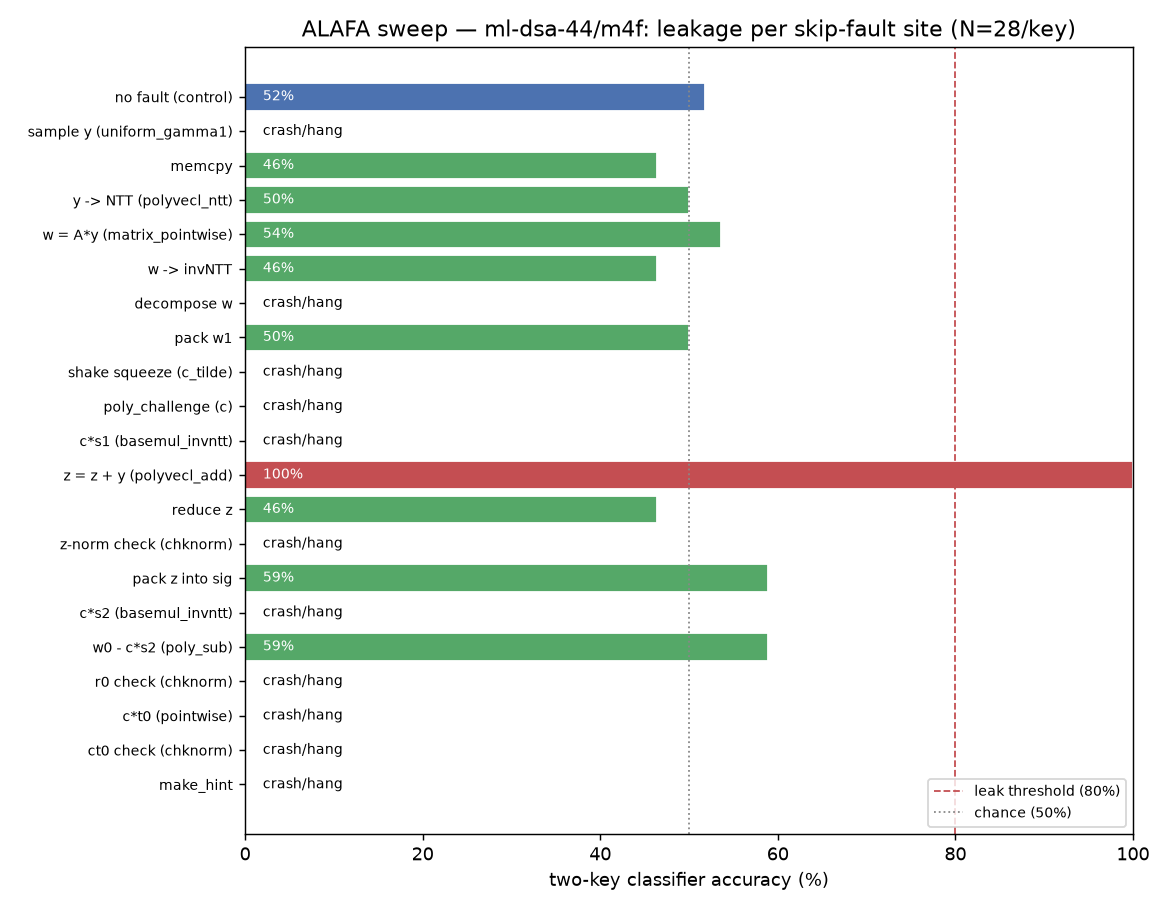
\includegraphics[width=0.82\textwidth]{../examples/plots/9/alafa_accuracy.png}}
  {\fbox{\parbox{0.8\textwidth}{\centering\itshape alafa\_accuracy.png ---
   the ALAFA sweep bar chart (one bar per site; red $=$ leak, grey $=$ crash/hang).}}}
\caption{ALAFA sweep verdict: only $z=z+y$ crosses; other sites crash/hang or sit at
chance.}
\label{fig:alafa}
\end{figure}

\begin{figure}[h]
\centering
\IfFileExists{../examples/plots/9/tvla_maxt.png}
  {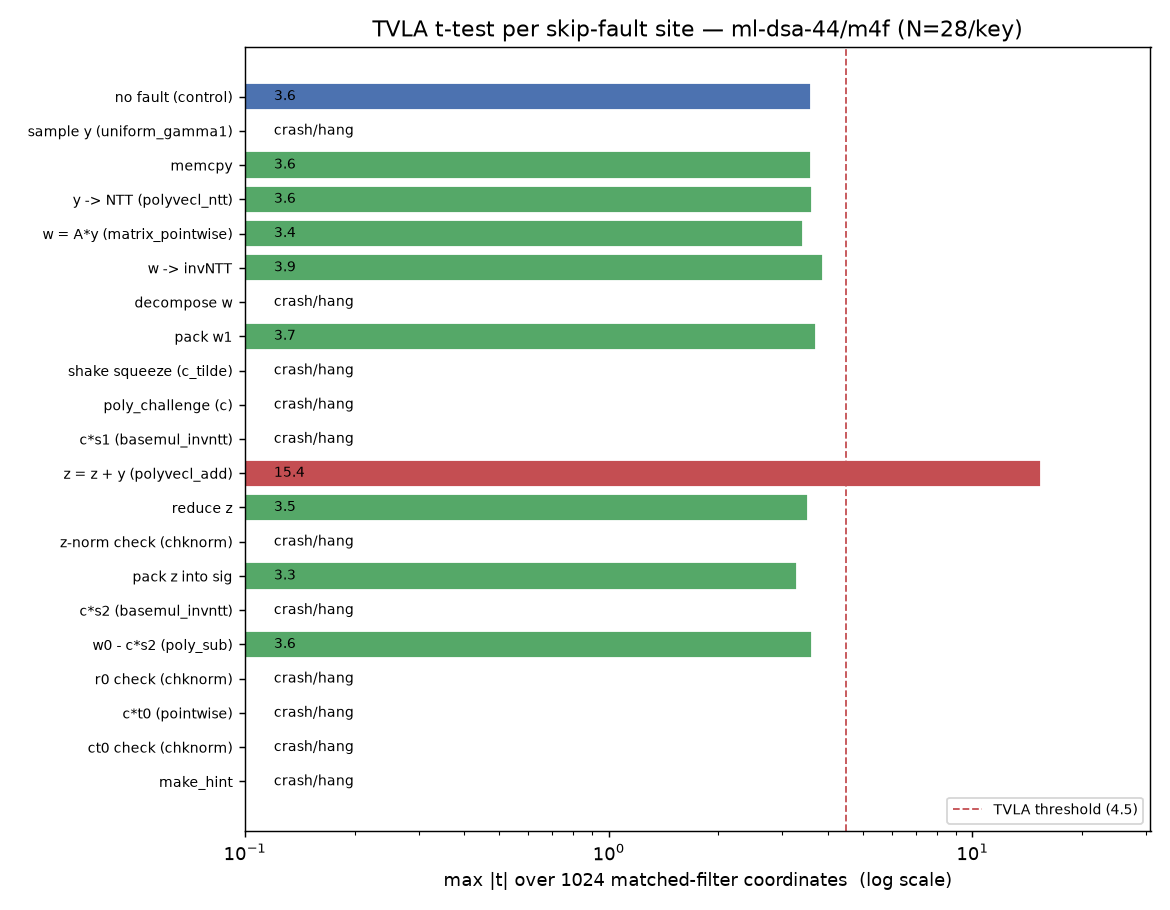
\includegraphics[width=0.72\textwidth]{../examples/plots/9/tvla_maxt.png}}
  {\fbox{\parbox{0.8\textwidth}{\centering\itshape tvla\_maxt.png --- per-site
   $\max|t|$ (log scale) with the $4.5$ threshold.}}}
\caption{TVLA twin of the verdict: only the mask-removal site rises above the
threshold.}
\label{fig:tvla}
\end{figure}

\paragraph{Why most sites hang.} A whole-call skip usually drops a value some
rejection check depends on, so the reject-and-retry loop \emph{never accepts} and
spins to the 20\,M-instruction cap. This is a real fault-model observation:
\emph{skipping a check and forcing its verdict are opposite faults}. Skipping
\code{bl poly\_chknorm} leaves a stale nonzero result $\to$ perpetual reject (hang);
the check-bypass \emph{leak} needs a stuck-at-accept data fault instead. So the
whole-call sweep is honestly scoped to high-SNR mask-removal faults.

\subsection{Auto-discovery: coverage versus cost}
Replacing the hand-authored 20-site table with disassembly-based discovery is a
strict \emph{superset}: all 20 curated sites appear among 48 discovered, and the one
leaking site is still flagged. The cost is a $\sim$5.7$\times$ slowdown
(Table~\ref{tab:alafa})---worse than the 48/20 site ratio predicts, because most of
the 28 extra sites are load-bearing setup calls whose skip makes signing hang to the
cap. The trade accepted: fully automatic, firmware-agnostic site generation in
exchange for more grey (hang) rows.

\begin{table}[h]
\centering\small
\caption{ALAFA sweep: coverage/cost of auto-discovery (ML-DSA-44, $N{=}12$/key).}
\label{tab:alafa}
\begin{tabular}{@{}lrrr@{}}
\toprule
Sweep & Sites & Leaks found & Wall time \\
\midrule
Curated table    & 20 & 1 ($z{=}z{+}y$) & 52.3\,s \\
Auto-discovered  & 48 & 1 ($z{=}z{+}y$) & 299.6\,s ($\sim$5.7$\times$) \\
\bottomrule
\end{tabular}
\end{table}

\subsection{Dilithium: intra-function skips (mode \code{funcskip})}
Inside \code{polyvecl\_add}, the calibrated \code{two\_key} detector flags exactly
two sites---the output-pointer load \code{0x46d2} and the mask add \code{0x46e4}---at
the permutation floor $p\approx 10^{-3}$, $\text{FDR}\le0.01$, with non-leaking sites
at $p\in[0.57,0.96]$. The \code{structural} detector flags the \emph{same} two sites
with $p=0$ (its degenerate-null tail) and \emph{no} false positives, every other
site sitting at $p=1.0$. Listing~\ref{lst:calib} shows the actual calibrated output;
the \code{--legacy-thresholds} run reproduces the same two sites via the old
$0.80$ cutoff.

\begin{lstlisting}[style=out,caption={Calibrated \code{funcskip} on ML-DSA-44
(\code{two\_key}). The p column and the FDR-based footer are the calibrated
verdict.},label={lst:calib}]
   addr  site                          metric      p  ran crash  status
  0x46d2  mov r7, r0                      100%  0.0010  16   0    LEAK  <- LEAK
  0x46d4  mov r6, r1                       50%  0.5684  16   0    ok
  0x46d6  mov r5, r2                       31%  0.8981  16   0    ok
  0x46e4  bl #0x3d94                      100%  0.0010  16   0    LEAK  <- LEAK
  0x46e8  cmp.w r4, #0x1000                25%  0.9600  16   0    ok
  -> 2 leaking site(s) at FDR<=0.01: 0x46d2 mov r7, r0, 0x46e4 bl #0x3d94
\end{lstlisting}

\subsection{LLVM-IR\,$\to$\,ARM translation and key-dependent ineffectiveness
($\varphi_{\mathrm{IF}}$)}\label{sec:llvmstudy}
Mapping the \textsc{Dilithium-LLVM} IR-level fault findings onto the compiled ARM
binary---\code{funcskip} over the $29$ reference functions, $n{=}40$ signatures per
key---sharpens two detector axes that must not be conflated: the \emph{correction}
axis (the faulted \emph{output distribution} differs by key: our \code{per\_coord}/TVLA
test) and the \emph{ineffective} axis (whether the skip is a \emph{no-op} differs by
key). On the correction axis only \code{polyvecl\_add} leaks ($5/10$ sites,
$\max|t|\approx16.9$ against a $3$--$4.5$ no-leak floor), so IR value-corruption
findings translate poorly to whole-instruction skips; and the \code{m4f} compiler
inlines $8$ reference functions (\code{polyveck\_add/sub/chknorm/make\_hint}, the
$c\cdot s$ \code{*\_pointwise\_poly\_montgomery} multiplies,
\code{polyvecl\_invntt}/\code{pointwise\_acc}) out of the signing path, shrinking the
fault surface below the IR the tool analysed.

The ineffective axis is the SIFA-style test $\varphi_{\mathrm{IF}}$: a
\emph{key-dependent} ineffective fault,
$\exists\,p\;\exists\,s_1,s_2:\ \Delta(\mathrm{fault}(s_1,p),\mathrm{gold}(s_1,p)){=}0
\,\wedge\, \Delta(\mathrm{fault}(s_2,p),\mathrm{gold}(s_2,p)){\neq}0$. We test it per
skip site with keys $A,B$ signing the \emph{same} message and signing-RNG (only
\code{sk} differs), counting \emph{flips}---messages where the skip is a no-op for one
key but output-changing for the other. This surfaces $71$ $\varphi_{\mathrm{IF}}$ sites
across four reachable functions (Table~\ref{tab:phiif}), where the earlier rate-based
\code{sifa} detector---comparing no-op \emph{rates} across unrelated signings---had
flagged none.

\begin{table}[h]
\centering\footnotesize
\caption{Key-dependent-ineffective ($\varphi_{\mathrm{IF}}$) sites on the ARM skip
surface, with the value that governs ineffectiveness. Only \code{ntt} is driven by a
\emph{hidden} quantity; the rest key on values that are public.}
\label{tab:phiif}
\begin{tabular}{@{}lrl@{}}
\toprule
Function & $\varphi_{\mathrm{IF}}$ sites (flips) & Governing value \\
\midrule
\code{ntt} & $63$ ($261$) & \textbf{secret-derived} (NTT of masked/secret polynomials) \\
\code{poly\_challenge} & $5$ ($7$) & \emph{public}: $\tilde c$, published in $\sigma$ \\
\code{polyvecl\_uniform\_gamma1} & $2$ ($38$) & secret: $y$ from $\rho'{=}H(K\,\|\,\mu)$ \\
\code{poly\_chknorm} & $1$ ($1$) & public-ish: norm check of $z$ \\
\bottomrule
\end{tabular}
\end{table}

Two observations qualify these counts. First, they are \emph{partial}: most sites flip
on only a handful of the $40$ messages, because a single-instruction skip is a no-op
only under a rare boundary condition---a redundant store, a dead write later
overwritten, an unused sign bit. At \code{poly\_challenge}'s coefficient store
\code{0x4122} the skip is \emph{effective} in $38/40$ messages for $A$ and $39/40$ for
$B$; a flip needs one key to hit the rare no-op where the other does not, which occurs
at just $3$ messages. Second---and more important for interpretation---the
``key-dependence'' is really \emph{input}-dependence: changing the key changes the
function's \emph{input}, and no-op-ness is a deterministic function of that input. For
\code{poly\_challenge} the input is the challenge seed $\tilde c = H(\mu\,\|\,w_1)$;
$w_1$ is secret-derived, so $A$ and $B$ feed \emph{different} $\tilde c$ (we confirm
$\mathrm{gold}_A\neq\mathrm{gold}_B$ at every message) and the no-op boundary falls at
different messages. But $\tilde c$ is \emph{published} in the signature
$\sigma=(\tilde c, z, h)$: the ineffectiveness depends on a value the attacker already
sees, so these sites are \emph{not} a secret oracle---they are SIFA false positives,
as is \code{poly\_chknorm} (keyed on the norm check of the near-public $z$). The one
surface where ineffectiveness tracks a \emph{hidden} quantity is \code{ntt}, whose
operands are the NTT of secret/masked polynomials that are not directly published; and
because the obvious $c\cdot s$ multiplies are inlined away, the genuine
key-dependent-ineffective surface lands there, on the Montgomery butterflies
(\code{smull}/\code{smlal}/\code{mul}/\code{add}). The corrected reading is therefore
not ``SIFA is absent on the skip surface'' but ``key-dependent ineffectiveness is
\emph{present} yet overwhelmingly \emph{public}-data-driven, with the NTT the lone
secret-relevant site.''

\subsection{MAYO: an honest negative result}
On MAYO the whole-call sweep finds \emph{zero} leaking sites, and this is the correct
answer for the current fault surface. The control sits at chance (46\%): fresh
vinegar masks the key just as $y$ does in Dilithium. Every vinegar-critical site
(SHAKE seed expansion, the linear solve, \code{compute\_M\_and\_VPV}) \emph{crashes}
under a whole-call skip, because zeroing the whole vinegar/seed makes the linear
solve fail; and the recombination $s=v+o$ is \emph{inlined}, so there is no
\code{bl} to skip. Even after rebuilding MAYO with the recombination de-inlined and
capturing it with \code{funcskip}, an instruction skip yields chance across all
detectors: the fused, word-vectorised \GF{16} loop exposes the \emph{vinegar}
operand (SHAKE-random, not separable), and the oil leak is \GF{16}-\emph{algebraic}.
What would flag it is a \emph{data fault} (zero/fix an operand) that leaves clean
oil, then the \GF{16} \code{structural} detector---the detector and localiser are in
place; the missing piece is wiring the data-fault model into the sweep. This is a
precise, useful negative result: it says exactly which capability the platform still
needs.

\subsection{Parallel speed and memory}
The MAYO sweep (heavily hang-dominated) runs in 566.8\,s serially and 37.4\,s at
\code{-j20}. As noted (\S\ref{sec:par}), threads cost $\approx$\,156\,MB against
$\approx$\,1.7\,GB for processes at the same width---the platform's central
parallelism tradeoff.

\subsection{Correctness}
The 32-test system suite passes on both standard CPython 3.12 and free-threaded
3.14t (with the GIL verified \emph{off}), and the \code{galois} oracle confirms the
hand-rolled \Zq{} and \GF{16} ranks against a trusted library. The calibration
change preserved every known verdict (the two \code{funcskip} sites, the ALAFA leak)
while removing the small-$N$ false positives.

\subsection{Positives and negatives, and the attacks they map to}\label{sec:posneg}
Table~\ref{tab:posneg} classifies the findings as \emph{positives} (a leak flagged)
or \emph{negatives} (nothing flagged), and names the published attack each positive
corresponds to --- so a detection reads as evidence for a concrete, documented fault
rather than an abstract score. The negatives are kept deliberately: a detector
framework earns trust from its honest misses as much as its hits. References are the
footnotes in Sections~\ref{sec:detectors}--\ref{sec:whysignal}.

\begin{table}[h]
\centering\footnotesize
\caption{Positives (a real leak flagged, with the corresponding published attack) and
negatives (nothing flagged, with the reason).}
\label{tab:posneg}
\begin{tabular}{@{}>{\raggedright\arraybackslash}p{3.5cm}>{\raggedright\arraybackslash}p{3.1cm}>{\raggedright\arraybackslash}p{5.1cm}@{}}
\toprule
Observation (site / fault) & Detector $\cdot$ result & Corresponding attack / reason \\
\midrule
\multicolumn{3}{@{}l}{\textbf{Positives --- a real leak, flagged}}\\
\addlinespace[2pt]
Mask removal $z=c\,s_1$ (skip \code{polyvecl\_add}) & \code{two\_key} 100\%, \code{structural} 0.92, \code{per\_coord} $|t|{=}12.9$ & ``Exploiting Determinism'' (Ravi \emph{et al.}); loop-abort (Espitau \emph{et al.}, SAC'16); Diff.\ Fault (Bruinderink--Pessl, CHES'18) \\
Out-of-spec accepted $r_0$ (forced accept, ex.\,08) & \code{spec\_aware} / \code{r0\_reject} & ``Finding a Polytope'' (PKC'25); the $r_0$-rejection bypass \\
Biased nonce $y$ (loop abort, \code{funcskip}) & \code{uniformity} & loop-abort / nonce-zeroing (Espitau \emph{et al.}) \\
Key-dependent ineffectiveness (planted) & \code{sifa} & SIFA (Dobraunig \emph{et al.}, 2018) \\
Key-dependent fault \emph{effect} (planted) & \code{differential} & differential fault analysis (general) \\
\midrule
\multicolumn{3}{@{}l}{\textbf{Negatives --- nothing flagged (honest), and why}}\\
\addlinespace[2pt]
MAYO skip sweep (any site) & all $\leq 54\%$ / $0.0$ $\to$ none & oil leak is \GF{16}-algebraic; needs a \emph{data} fault exposing clean oil, then \code{structural} over \GF{16} \\
\code{sifa} / \code{r0\_reject} on the skip surface & $0$ flagged & need the data-fault surface (\code{SET\_MEM}/\code{BITFLIP}); skip-only hangs or yields no $r_0$ \\
\code{poly\_chknorm} skip & crash/hang & stale verdict $\to$ infinite reject loop (not a leak) \\
\code{per\_coord}/TVLA at the unfaulted control & $p\approx0.007$ (false positive) & small-$N$ normal tail is anti-conservative; tolerated for a detector framework \\
\code{differential} / \code{sifa} across the skip sweep & $0$ new after FDR & the skip surface's only secret leak is the mask removal (\code{two\_key}'s); the direct $\varphi_{\mathrm{IF}}$ reading (\S\ref{sec:llvmstudy}) finds key-dependent ineffectiveness present but public-data-driven except in the NTT \\
\bottomrule
\end{tabular}
\end{table}

%======================================================================
\section{Design Tradeoffs}\label{sec:tradeoffs}
%======================================================================

\begin{description}[leftmargin=0em,style=nextline]
\item[Emulation vs.\ hardware.] Emulation gives perfect determinism, full
observability, byte-identical firmware, and cheap snapshot/restore---at the cost of
not modelling analogue effects (partial glitches, timing, EM). \ucpqc{} embraces
this: it is a \emph{fault-effect} analyser (``does this logical fault re-open a
channel?''), not a physical side-channel simulator. It cleanly models the digital
consequence of a glitch (skip / bit-flip / stuck-at) and is explicit that a
\emph{partial} nonce abort (Dilithium category 4.1) is outside the whole-call model.

\item[Leak-detection vs.\ key recovery.] Deciding leak/no-leak needs tens of
traces and yields an interpretable verdict; full key recovery needs many signatures
and heavier cryptanalysis. The platform picks the former deliberately, which is what
makes an exhaustive per-site sweep affordable.

\item[Whole-call \code{sweep} vs.\ \code{funcskip}.] \code{sweep} is coarse but
needs no target description and covers the whole loop; \code{funcskip} is fine-grained
(every instruction) and $\sim$240$\times$ cheaper per trial, but needs a
\code{Target} (arg layout) and can surface isolated-replay artefacts (e.g.\ the
\code{0x46d2} pointer-aliasing site) that a full signing would overwrite.

\item[Auto-discovery vs.\ curated sites.] Disassembly-based sites are zero-config and
a strict coverage superset, at $\sim$5.7$\times$ runtime because most extra sites
hang to the instruction cap. Coverage and portability were judged worth the cost.

\item[Calibrated $p$-values vs.\ fixed thresholds.] Calibration gives every verdict a
false-discovery guarantee and removes per-scheme tuning; the cost is the permutation
compute and the empirical floor $1/(n_{\text{perm}}+1)$, which for wide-null
classifiers means $n_{\text{perm}}$ must scale with site count. The design mitigates
this with a Gaussian-tail refinement that is sharp exactly for the structural
detector (whose leaks are most often isolated), and keeps \code{--legacy-thresholds}
for reproducibility.

\item[Hand-rolled vs.\ library math.] The bug-prone \Zq{} NTT was replaced by
\code{sympy}; the small finite-field ranks were kept in numpy (fast, on the hot path)
but are oracle-tested against \code{galois}. The binding constraint is
free-threading: every runtime dependency must be pure-Python or GIL-safe, so
\code{galois}/\code{numba} are test-only.

\item[Processes vs.\ free threads.] Processes are simple and robust (no shared C
state) but cost $\sim$11$\times$ the memory; free threads are memory-frugal but
require CPython 3.14t and a GIL-safe dependency set. The platform keeps both on
rebase-friendly branches so the choice is the operator's.
\end{description}

%======================================================================
\section{Limitations and Future Work}\label{sec:future}
%======================================================================

The audit identified four extension axes; the first has been built.

\begin{enumerate}[leftmargin=1.5em]
  \item \textbf{Calibrated detectors} \emph{(done, branch \code{calibrated-detectors})}
  --- \S\ref{sec:calib}.
  \item \textbf{Fault-model sweep.} The detector sweep currently injects only
  \code{SKIP}; the six-model injector (\code{SET\_MEM}, \code{BITFLIP\_*},
  \code{FLIP\_FLAGS}) exists but is wired only to the golden-comparison campaign.
  Unifying them would let the detector repertoire run over data-corruption and
  branch-inversion faults---directly enabling MAYO vinegar-zeroization and
  seed-fixing, and Dilithium check-bypass, which the skip-only sweep cannot express.
  \item \textbf{ML-KEM profile.} The KEM scheme layer and \code{ml-kem-768} firmware
  are present but no profile drives them; adding one proves genericity across the
  SIGN/KEM axis and exercises the detectors on Kyber decapsulation faults.
  \item \textbf{Known-answer matrix + protected-vs-unprotected diff.} Pin each
  documented attack to an expected calibrated verdict (true-positive and golden
  true-negative), and add a mode that runs the same sweep on a hardened and an
  unprotected ELF, reporting which leaks a countermeasure closes, leaves, or newly
  introduces---the named use case.
\end{enumerate}

Other known limits: \code{structural} \code{funcskip} is slow ($\sim$3--4\,min) due
to the per-signature \code{sympy} ring deconvolution in featurisation (not the
calibration); and for very large classifier sweeps with an isolated leak,
$n_{\text{perm}}$ should be raised until the floor clears $q/m$.

%======================================================================
\section{Conclusion}
%======================================================================

\ucpqc{} is a compact ($\sim$5.3\,k LoC) but complete platform for systematic,
emulation-based fault-leakage analysis of PQC firmware. Its layered design confines
scheme knowledge to a thin profile layer, so the emulator, fault injector,
capture-replay engine, detector repertoire, and now the statistical calibration are
all reused unchanged across lattice and multivariate schemes. The recent calibration
work turns every \textsc{leak} verdict into a permutation- or analytically-derived
$p$-value with a sweep-wide false-discovery guarantee, eliminating four magic
thresholds and any per-scheme tuning, while preserving every validated detection.
The results are faithful in both directions: the platform pinpoints Dilithium's
mask-removal leak at 100\% (and its calibrated $p\approx10^{-3}$ / structural $p=0$),
and it reports an honest negative on MAYO that names the exact missing capability---a
data-fault sweep---as the next step.

\appendix
%======================================================================
\section{CLI Reference}
%======================================================================
\begin{lstlisting}[style=sh]
python -m ucpqc info      fw.elf                 # scheme binding + memory map
python -m ucpqc roundtrip fw.elf                 # one keygen/sign/verify (or KEM) cycle
python -m ucpqc sweep     fw.elf --n 24          # whole-call leak sweep (ALAFA)
python -m ucpqc funcskip  fw.elf --target polyvecl_add   # intra-function skip sweep
python -m ucpqc fault     fw.elf --func challenge --model set_mem   # golden-comparison campaign
# calibration flags (sweep / funcskip):
#   --detector two_key|per_coord|subspace|structural|mmd|uniformity|spec_aware
#   --n-perm 1000  --fdr 0.01  --correction bh|holm  --legacy-thresholds
\end{lstlisting}

%======================================================================
\section{Test and Verification Summary}
%======================================================================
\begin{itemize}[leftmargin=1.4em]
  \item 32 system tests (\code{tests/run\_tests.py}) --- pass on CPython 3.12 and
  free-threaded 3.14t (GIL verified off).
  \item Field oracle (\code{tests/test\_field\_oracle.py}) --- \Zq{} and \GF{16}
  ranks matched against \code{galois} (3.12 only).
  \item Calibration self-tests --- permutation calibration and generalisation,
  Benjamini--Hochberg / Holm control, and the \code{per\_coord} $p$-value/threshold
  duality.
  \item Regression --- calibrated verdicts reproduce the two \code{funcskip} leak
  sites and the ALAFA leak; \code{--legacy-thresholds} reproduces the pre-calibration
  results.
\end{itemize}

\end{document}
